%-----------------------------------------------------------------------------
%
%               Template for sigplanconf LaTeX Class
%
% Name:         sigplanconf-template.tex
%
% Purpose:      A template for sigplanconf.cls, which is a LaTeX 2e class
%               file for SIGPLAN conference proceedings.
%
% Guide:        Refer to "Author's Guide to the ACM SIGPLAN Class,"
%               sigplanconf-guide.pdf
%
% Author:       Paul C. Anagnostopoulos
%               Windfall Software
%               978 371-2316
%               paul@windfall.com
%
% Created:      15 February 2005
%
%-----------------------------------------------------------------------------


\documentclass[preprint]{sigplanconf}

% The following \documentclass options may be useful:

% preprint      Remove this option only once the paper is in final form.
% 10pt          To set in 10-point type instead of 9-point.
% 11pt          To set in 11-point type instead of 9-point.
% authoryear    To obtain author/year citation style instead of numeric.

\usepackage{amsmath,amssymb}
\usepackage[T1]{fontenc}
\usepackage[utf8]{inputenc}
\usepackage{filecontents}
\usepackage{hyperref}
\usepackage{graphicx}
\usepackage{float}

\usepackage[os=win]{menukeys}
\renewmenumacro{\keys}{shadowedroundedkeys}

\hypersetup{breaklinks=true,
            bookmarks=true,
            pdfauthor={},
            pdftitle={},
            colorlinks=true,
            citecolor=blue,
            urlcolor=blue,
            linkcolor=blue,
            pdfborder={0 0 0}}

\newlength{\almostverbatimindentation}
\newenvironment{almostverbatim}{%
\sbox0{\texttt{\global\almostverbatimindentation=2\fontdimen2\font}}
\\[\topsep]\hspace*{\almostverbatimindentation}\begin{minipage}{0.94\linewidth}\setlength{\baselineskip}{1.5\baselineskip}%
}{%
\end{minipage}\\[\topsep]
}

\begin{filecontents}{workshop.bib}
@Manual{Coq,
  title =        {The {Coq} Proof Assistant Reference Manual},
  author =       {{The Coq Development Team}},
  organization = {{LogiCal} Project},
  note =         {Version 8.0},
  year =         {2004},
  url =          "http://coq.inria.fr"
}

@InCollection{ProofGeneral,
  Title                    = {{Proof General: A Generic Tool for Proof Development}},
  Author                   = {Aspinall, David},
  Booktitle                = {Tools and Algorithms for the Construction and Analysis of Systems, {TACAS} 2000},
  Publisher                = {Springer Berlin Heidelberg},
  Year                     = {2000},
  Editor                   = {Graf, Susanne and Schwartzbach, Michael},
  Pages                    = {38--43},
  Series                   = {Lecture Notes in Computer Science},
  Volume                   = {1785},
  Doi                      = {10.1007/3-540-46419-0_3},
  ISBN                     = {978-3-540-67282-1},
  Language                 = {English},
  Url                      = {http://dx.doi.org/10.1007/3-540-46419-0_3}
}

@Misc{SMIE,
  Title                    = {{SMIE}: {S}imple {M}inded {I}ndentation {E}ngine},
  Author                   = {Stefan Monnier},
  Url                      = {https://www.gnu.org/software/emacs/manual/html_node/elisp/SMIE.html},
  Year                     = {2010}
}
\end{filecontents}

\usepackage{xspace}
% To have the same capitalization everywhere
\newcommand{\proofg}{Proof General\xspace}
\begin{document}

\special{papersize=8.5in,11in}
\setlength{\pdfpageheight}{\paperheight}
\setlength{\pdfpagewidth}{\paperwidth}

\conferenceinfo{CoqPL 2016}{January 23, 2016, St. Petersburg, Florida, United States}
\copyrightyear{2016}
% \copyrightdata{978-1-nnnn-nnnn-n/yy/mm}
% \doi{nnnnnnn.nnnnnnn}

% Uncomment one of the following two, if you are not going for the 
% traditional copyright transfer agreement.

%\exclusivelicense                % ACM gets exclusive license to publish, 
                                  % you retain copyright

%\permissiontopublish             % ACM gets nonexclusive license to publish
                                  % (paid open-access papers, 
                                  % short abstracts)

\titlebanner{}        % These are ignored unless
\preprintfooter{Company-Coq: Taking \proofg one step closer to a real IDE}   % 'preprint' option specified.

\title{Company-Coq: Taking \proofg one step closer to a real IDE}
\subtitle{A tutorial on using \proofg and its new extension to write proofs more efficiently}

\authorinfo{Cl\'ement Pit-Claudel}
           {MIT CSAIL}
           {cpitcla@mit.edu}
\authorinfo{Pierre Courtieu}
           {CNAM, Lab. C\'edric}
           {pierre.courtieu@cnam.fr}

\maketitle

\begin{abstract}
\texttt{Company-Coq} is a new Emacs package that extends \proofg with a contextual auto-completion engine for Coq proofs and many additional facilities to make writing proofs easier and more efficient. Beyond fuzzy auto-completion of tactics, options, module names, and local definitions, \texttt{company-coq} offers offline in-editor documentation, convenient snippets, and multiple other Coq-specific IDE features. The presentation will focus on a live demo of the system with an emphasis on writing proofs in Emacs more efficiently, and a discussion of desirable features of proof-oriented development environments.
\end{abstract}

\category{D.2.6}{Software Engineering}{Programming Environments---Integrated environments}

\keywords IDE, documentation, proof engineering, user experience

\section*{Introduction}

Users of the Coq Proof Assistant \cite{Coq} are roughly divided between two interactive development environments\footnote{There also exist Coq interfaces for vim and Eclipse, though their use does not seem very widespread.}: \emph{\proofg}, an extension of Emacs written by David Aspinall \cite{ProofGeneral}, and \emph{CoqIDE}, a Coq-specific development environment written from scratch by members of the Coq team and generally touted as more beginner-friendly (mostly due to \proofg's dependence on Emacs). Both are powerful tools for writing proofs, and significantly improve the experience of proof authors when compared to Coq's simple read-eval-print loop. Yet these tools do not offer advanced features typically found in IDEs, such as in-editor documentation or context-sensitive completion. In addition, when advanced features are in fact available (\proofg, for example, does supports snippets and improved display of mathematics), they tend to lack discoverability: users do not explore the menus and miss convenient features that would make them more efficient.

\href{https://github.com/cpitclaudel/company-coq/}{\texttt{Company-Coq}} is a new Emacs package that attempts to fix some of these limitations: we extend \proofg with many advanced IDE features (fuzzy completion, various Coq-specific snippets, and in-editor documentation for most of Coq's 2000-odd tactics, options, and errors), and solve the discoverability issue by taking an ``all-on'' approach: the default distribution has most features automatically enabled\footnote{For example, although \proofg does support enhanced displaying of mathematics (non-destructively displaying \texttt{fun (n m: nat) => forall p, p <> n -> p >= m} as \texttt{$\lambda$ (n m: $\mathbb{N}$) $\Rightarrow$ $\forall$ p, p $\neq$ n $\rightarrow$ p $\geq$ m}), few users seem to know about this feature. \texttt{Company-Coq}, on the other hand, enables a similar feature by default, and most users seem pleased with it.}. In addition, \texttt{company-coq} comes with a comprehensive tutorial that showcases most of its features.
Since it is not part of the core \proofg, \texttt{company-coq} can serve as a convenient experimentation area for new features and development directions, before they are merged into other IDEs.%\proofg or CoqIDE.

\section*{Workshop description}

The presentation will consist of a quick run through \texttt{company-coq}'s features, and a tutorial on using these and other \proofg features to write proofs more efficiently with emphasis on the lemma extraction feature. The workshop will also be a good occasion to showcase some features that \proofg inherits from Emacs, to discuss how much of this work could be used to enhance other Coq interfaces, and to ponder about desirable features for proof-oriented development environments.

\section*{Overview of some features of \texttt{company-coq}}

\paragraph{Context-sensitive autocompletion with holes} \texttt{Company-Coq} implements a number of backends for the \href{https://company-mode.github.io/}{\emph{CompleteAnything}} Emacs package (\texttt{company}). Typing \texttt{app{\kern0.5pt}in} therefore suggests variants of the apply tactic (bold text indicates holes):

\begin{figure}[H]
  \centering
  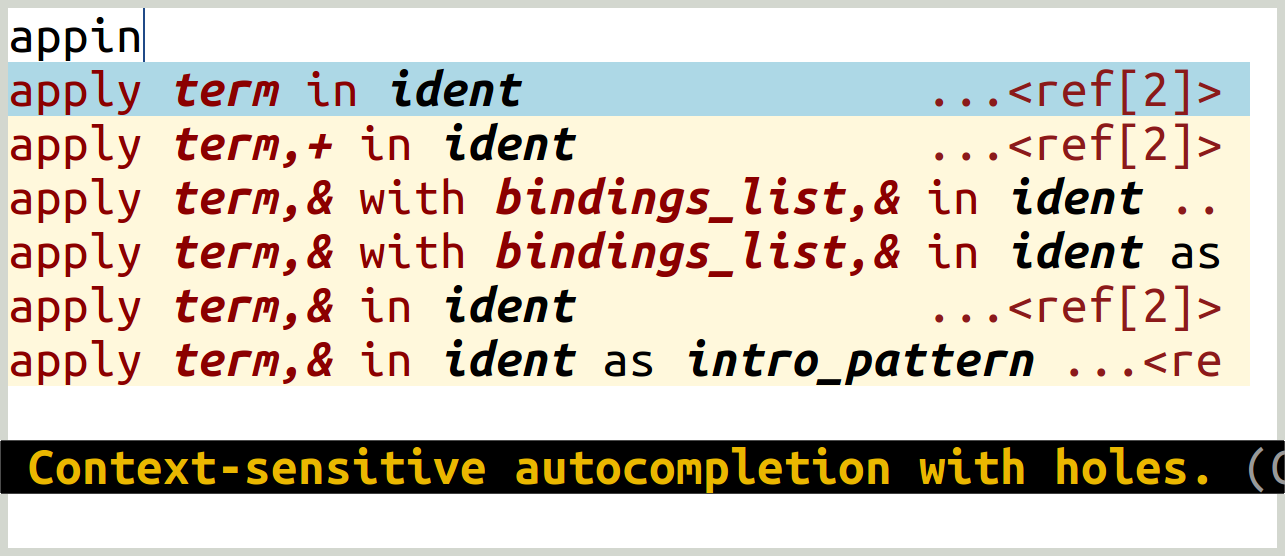
\includegraphics[width=\linewidth]{coq-pl-16-autocompletion.png}
\end{figure}

\paragraph{Offline documentation} Part of the development of
\texttt{company-coq} involved cross-referencing tactics and options
from the user manual; this allows \texttt{company-coq} to display
documentation for most completion entries, without querying INRIA's
website\footnote{The list of tactic templates, and the associated
  documentation, is extracted from the annotated manual into an index and a set of data files that could be useful to other editors.}:

\begin{figure}[H]
  \centering
  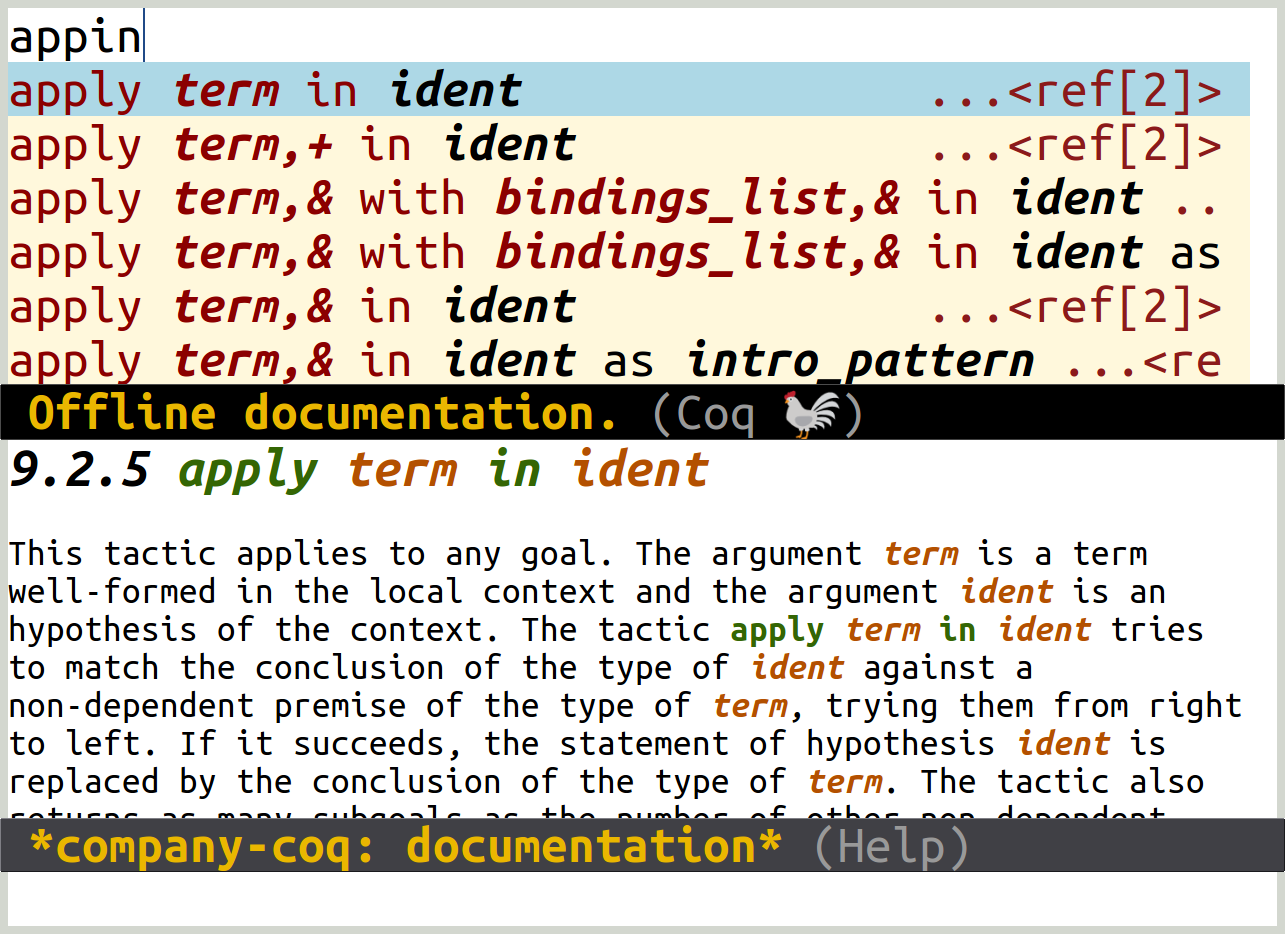
\includegraphics[width=\linewidth]{coq-pl-16-documentation.png}
\end{figure}

\paragraph{Lemma extraction} At any point in a proof, users may choose to extract the current goal, including some hypotheses, to a separate lemma. Instead of painstakingly copy-pasting bits of the proof context, \texttt{company-coq} offers a convenient interface to pick hypotheses and generate the statement of the extracted lemma\footnote{The statement is produced by generalizing the hypotheses that the goal mentions and the ones that the user selected, using a small Ltac script.}.

\paragraph{Point and click documentation} Clicking on an identifier while
pressing the control key opens an inline documentation window (which disappears
when the mouse button is released):

\begin{figure}[H]
  \centering
  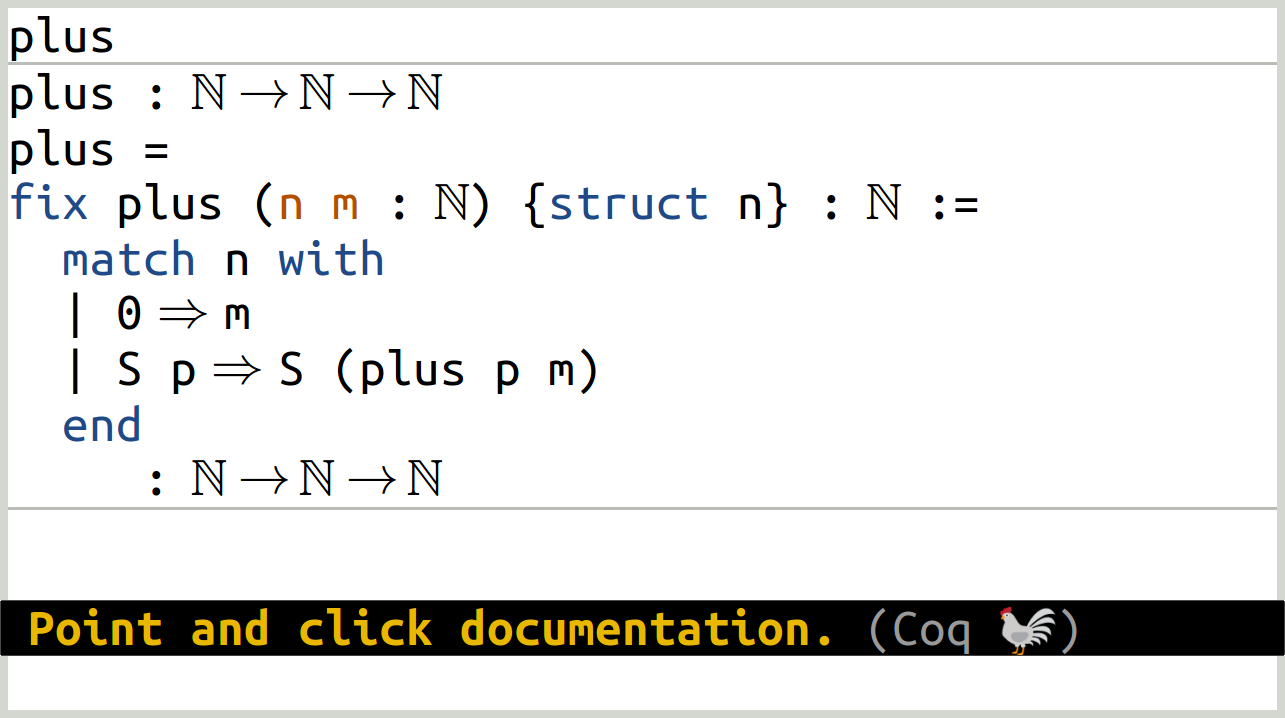
\includegraphics[width=\linewidth]{coq-pl-16-point-and-click.png}
\end{figure}

\paragraph{Snippets} \texttt{Company-Coq} connects with \texttt{YASnippet} to make certain common Coq patterns quicker to write. For example, to write
\begin{verbatim}
  match goal with
  | [ H: ?a /\ ?b |- ?a ] => destruct H; assumption
  end
\end{verbatim}
the user only needs to type the following commands:
\begin{almostverbatim}
  \verb|m g w | \keys{\return}\\
  \keys{\Alt+\shift+\return} \verb| | \keys{\tab} \verb| ?a /\ ?b | \keys{\tab} \verb| ?a | \keys{\tab}\\
  \verb|destr | \keys{\return} \verb| H; ass | \keys{\return}
\end{almostverbatim}
The key here is the \keys{\Alt+\shift+\return} shortcut, which introduces the
\begin{verbatim}
  | [ H: _ |- _ ] => _
\end{verbatim}
pattern, leaving holes that the user can navigate between with \texttt{TAB} in place of each \texttt{\_}.

\paragraph{Automatic named introduction} Scripts that depend on the names of hypotheses can often be made more robust by choosing names explicitly: \texttt{company-coq} leverages an existing feature of \proofg to let the user type
\begin{almostverbatim}
  \verb|intros! |\keys{\return}
\end{almostverbatim}
to create an invocation of the \texttt{intros} tactic that explicitly mentions all introduced variables.

\section*{New features of \proofg}

A number of new \proofg features are also useful for proof development:

\paragraph{Automatic indentation of bulleted proofs} Coq proofs can be structured with \emph{bullets} and curly brackets, making proof structure more readily apparent, and helping with maintenance. Thanks to \texttt{SMIE} \cite{SMIE}, \proofg implements an indentation routine based on structuring commands which makes proofs easier to format.

\paragraph{Automatic recompilation at \texttt{Require}} When developing a proof, one has to deal with several inter-dependent files. \proofg, thanks to a contribution of Hendrik Tews, can transparently and recursively recompile dependencies as it reaches \texttt{Require} commands, launching the required compilation jobs in the background.

% Je laisse ça de côté vu aue ce n'est pas encore implémenté dans Company-Coq :)
% In the same spirit some tactics come with the ability to name the created hypothesis (\texttt{induction ... as ..., inversion ... as ..., \ldots}) \proofg comes with a facility to automatically generate the \texttt{as} closes and \texttt{Company-Coq}\marginote{\`a implanter/changer} bring this feature to the user as an auto-completion of the keyword \texttt{as!}.

\section*{Conclusion}
\texttt{Company-Coq} has been well received by the community\footnote{At this time, \texttt{company-coq} has accumulated \href{http://melpa.org/\#/company-coq}{750 downloads}.}, and we expect many of its features to find their way into other Coq development environments\footnote{Indeed, the architecture of company-coq should be amenable to such cross-pollination: none of its features are Emacs-specific, and the collection of pre-processing scripts that it relies on to offer documentation, completion and snippets is freely available (along with their output).}; we hope that the CoqPL workshop will be a good venue to discuss it, and more generally to discuss the development of new editor features enhancing the experience of authors of Coq programs and proofs.

\bibliographystyle{abbrvnat}
\bibliography{workshop}

\end{document}
